\documentclass[12pt,a4paper]{article}
\usepackage{amsmath, amssymb, geometry, booktabs, xcolor, hyperref,
            listings, pgfplots, tcolorbox, enumitem, fancyhdr, tikz, array}
\geometry{margin=2.5cm}
\pgfplotsset{compat=1.18}
\tcbuselibrary{skins, breakable}

% ── tcolorbox environments ──────────────────────────────────────────────────
\newtcolorbox{curiositybox}[1]{colback=yellow!10, colframe=orange!80!black,
  fonttitle=\bfseries, title=#1, breakable}
\newtcolorbox{infobox}[1]{colback=blue!5, colframe=blue!60!black,
  fonttitle=\bfseries, title=#1, breakable}
\newtcolorbox{mistakebox}[1]{colback=red!5, colframe=red!60!black,
  fonttitle=\bfseries, title=#1, breakable}
\newtcolorbox{learnbox}[1]{colback=green!5, colframe=green!60!black,
  fonttitle=\bfseries, title=#1, breakable}

% ── listings (Python) ───────────────────────────────────────────────────────
\lstset{language=Python, basicstyle=\ttfamily\small, keywordstyle=\color{blue},
        commentstyle=\color{gray}, stringstyle=\color{orange},
        showstringspaces=false, numbers=left, numberstyle=\tiny,
        breaklines=true, frame=single}

% ── fancyhdr ────────────────────────────────────────────────────────────────
\pagestyle{fancy}
\fancyhf{}
\lhead{Topic 11: Division by t}
\rhead{Unit IV --- Laplace Transforms}
\cfoot{\thepage}

% ── title ───────────────────────────────────────────────────────────────────
\title{Topic 11: Division by t \\ \large Unit IV --- Laplace Transforms}
\author{23A54201 --- Mathematics IV (Transform Techniques)\\
        JNTUA College of Engineering (Autonomous)}
\date{}

% ============================================================================
\begin{document}
\maketitle
\tableofcontents
\newpage

% ============================================================================
\section{Opening Hook}

\begin{curiositybox}{Hook}
In Topic 10, you discovered that multiplying $f(t)$ by $t$ differentiates $F(s)$.
Now the beautiful mirror image: dividing $f(t)$ by $t$ integrates $F(s)$ from
$s$ to $\infty$. This gives you the transform of functions like $\sin(t)/t$ ---
a function that appears in communication theory (the sinc function) and is
famously difficult to integrate directly. With the division-by-$t$ property,
its Laplace transform is just
\[
  \int_s^\infty \frac{1}{u^2+1}\,du \;=\; \frac{\pi}{2} - \arctan(s).
\]
Elegant, fast, and powerful.
\end{curiositybox}

% ============================================================================
\section{Why This Topic Exists}

``Before we begin, here is the honest answer to why you are reading this\ldots''
Functions divided by $t$ appear throughout applied mathematics and engineering.
The sinc function $\sin(t)/t$ is the impulse response of an ideal low-pass
filter in signal processing. The ratio $(e^{at}-e^{bt})/t$ appears in heat-flow
problems and integral evaluations. Without the division-by-$t$ property we would
be forced into difficult direct integrations; with it the answer is one clean
integral of $F(s)$ in the $s$-domain.

\medskip
\begin{center}
\begin{tabular}{@{}ll@{}}
\toprule
\textbf{Mistake} & \textbf{Consequence} \\
\midrule
Not checking the existence condition $\lim_{t\to 0^+} f(t)/t$ &
  Applying the formula to a non-integrable function and getting wrong results \\[4pt]
Integrating from $0$ to $s$ instead of $s$ to $\infty$ &
  Completely wrong answer --- direction of integration matters \\[4pt]
Confusing with the integral transform formula (Topic 09) &
  Using $F(s)/s$ instead of $\int_s^\infty F(u)\,du$ \\
\bottomrule
\end{tabular}
\end{center}

\begin{learnbox}{Key Warning}
Always verify the existence condition \emph{before} applying
$\mathcal{L}\!\left\{\dfrac{f(t)}{t}\right\} = \int_s^\infty F(u)\,du$.
The integration runs from $s$ up to $\infty$, not the other way.
\end{learnbox}

% ============================================================================
\section{You Already Know This (Intuition First)}

Recall from ordinary calculus that differentiation and integration are
inverse operations. The same elegant duality appears in the Laplace world:
\begin{itemize}[leftmargin=2em]
  \item \textbf{Multiply by $t$} in the time domain $\longleftrightarrow$
        \textbf{differentiate} $F(s)$ (Topic 10).
  \item \textbf{Divide by $t$} in the time domain $\longleftrightarrow$
        \textbf{integrate} $F(s)$ from $s$ to $\infty$ (this topic).
\end{itemize}

Just as integration ``un-differentiates'' a function, dividing by $t$
``un-differentiates'' in the $s$-domain --- it recovers the integral of $F(s)$
from $s$ to $\infty$. This Topics 10--11 duality mirrors the derivative-integral
duality you already know, making the new formula easy to remember:
\emph{multiply $\to$ differentiate; divide $\to$ integrate}.

% ============================================================================
\section{The Main Theorem --- Division by t}

\begin{infobox}{Theorem: Division by $t$}
\textbf{Theorem.}\;
If $\mathcal{L}\{f(t)\} = F(s)$ and $\displaystyle\lim_{t \to 0^+}
\frac{f(t)}{t}$ exists (is finite), then
\[
  \mathcal{L}\!\left\{\frac{f(t)}{t}\right\} = \int_s^\infty F(u)\,du.
\]

\textbf{Proof.}\;
Start from the definition of $\int_s^\infty F(u)\,du$:
\[
  \int_s^\infty F(u)\,du
  = \int_s^\infty \left[\int_0^\infty e^{-ut}\,f(t)\,dt\right] du.
\]
Both iterated integrals converge absolutely (since $f$ is of exponential order
and the existence condition guarantees no singularity at $t=0$), so Fubini's
theorem permits interchange of order:
\[
  = \int_0^\infty f(t)\left[\int_s^\infty e^{-ut}\,du\right] dt.
\]
Evaluate the inner integral: for $t > 0$ and $\operatorname{Re}(s) > 0$,
\[
  \int_s^\infty e^{-ut}\,du
  = \left[\frac{e^{-ut}}{-t}\right]_s^\infty
  = 0 - \frac{e^{-st}}{-t}
  = \frac{e^{-st}}{t}.
\]
Substituting back:
\[
  \int_s^\infty F(u)\,du
  = \int_0^\infty f(t)\cdot\frac{e^{-st}}{t}\,dt
  = \int_0^\infty e^{-st}\,\frac{f(t)}{t}\,dt
  = \mathcal{L}\!\left\{\frac{f(t)}{t}\right\}. \qquad\square
\]

\textbf{Existence Condition.}\;
The theorem requires $\displaystyle\lim_{t \to 0^+}\frac{f(t)}{t}$ to be
finite. If $f(0)\neq 0$, then $f(t)/t \sim f(0)/t \to \infty$ as $t\to 0^+$
and the Laplace integral diverges. Consequently we need $f(0)=0$ (or more
precisely, $\lim_{t\to 0^+}f(t)/t$ finite). For example,
$\mathcal{L}\{\cos(t)/t\}$ does \textbf{not} exist because
$\cos(0)/0 \to \infty$.
\end{infobox}

\begin{learnbox}{What Did We Learn?}
$\mathcal{L}\!\left\{f(t)/t\right\} = \int_s^\infty F(u)\,du$, proved by
swapping integration order via Fubini. The existence condition $f(0)=0$ is
non-negotiable.
\end{learnbox}

% ============================================================================
\section{Key Application --- \texorpdfstring{$\mathcal{L}\{\sin(t)/t\}$}{L{sin(t)/t}}}

\begin{infobox}{Derivation: $\mathcal{L}\{\sin(t)/t\}$}
Let $f(t) = \sin t$. Then $\mathcal{L}\{\sin t\} = F(s) = \dfrac{1}{s^2+1}$.

\textbf{Check existence condition:}
$\displaystyle\lim_{t\to 0^+}\frac{\sin t}{t} = 1$ (finite). \checkmark

\textbf{Apply the theorem:}
\[
  \mathcal{L}\!\left\{\frac{\sin t}{t}\right\}
  = \int_s^\infty \frac{du}{u^2+1}
  = \Big[\arctan(u)\Big]_s^\infty.
\]
Now evaluate the limits:
\[
  \lim_{u\to\infty}\arctan(u) = \frac{\pi}{2}, \qquad
  \arctan(s)\text{ at the lower limit}.
\]
Therefore:
\[
  \mathcal{L}\!\left\{\frac{\sin t}{t}\right\}
  = \frac{\pi}{2} - \arctan(s).
\]
\end{infobox}

\medskip
\noindent\textbf{Graph of the sinc function $f(t)=\sin(t)/t$.}

\begin{center}
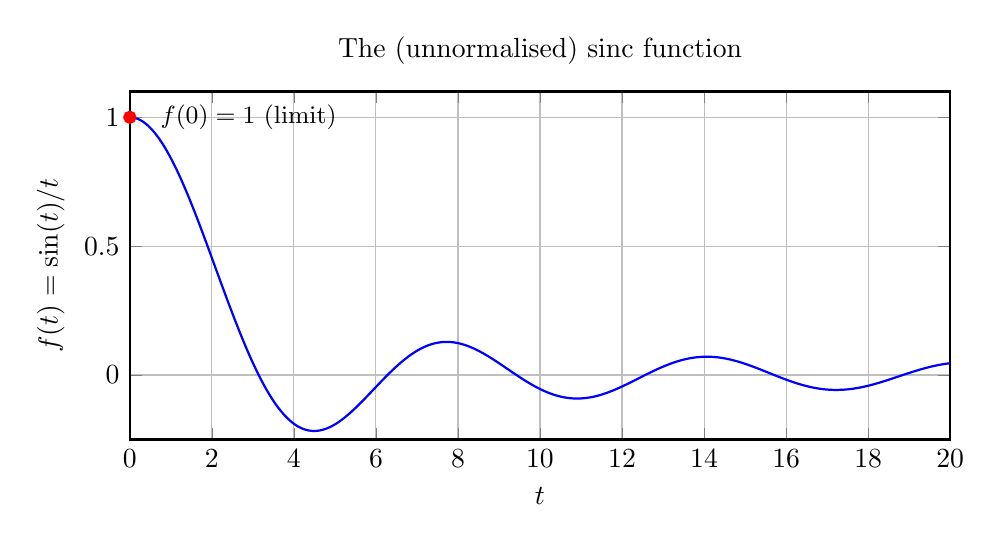
\begin{tikzpicture}
\begin{axis}[
  xlabel={$t$},
  ylabel={$f(t) = \sin(t)/t$},
  title={The (unnormalised) sinc function},
  xmin=0, xmax=20,
  ymin=-0.25, ymax=1.1,
  grid=major,
  width=12cm, height=6cm,
  samples=400,
  domain=0.001:20,
  thick
]
\addplot[blue, thick] {sin(deg(x))/x};
\addplot[dashed, red, domain=0:20] coordinates {(0,1)(0.001,1)};
% f(0)=1 by the limit
\addplot[mark=*, mark size=2pt, red] coordinates {(0,1)};
\node[right] at (axis cs: 0.5, 1) {\small $f(0)=1$ (limit)};
\end{axis}
\end{tikzpicture}
\end{center}

\begin{learnbox}{What Did We Learn?}
$\mathcal{L}\!\left\{\dfrac{\sin t}{t}\right\} = \dfrac{\pi}{2} - \arctan(s)$.
The key steps: (1) recognise $F(s)=1/(s^2+1)$, (2) verify the existence
condition, (3) integrate and evaluate using $\arctan(\infty)=\pi/2$.
\end{learnbox}

% ============================================================================
\section{Key Application --- \texorpdfstring{$\mathcal{L}\{(e^{at}-e^{bt})/t\}$}{L{(e^at-e^bt)/t}}}

\begin{infobox}{Derivation: $\mathcal{L}\{(e^{at}-e^{bt})/t\}$}
Let $f(t) = e^{at} - e^{bt}$ (assume $s > \max(a,b)$ for convergence). Then
\[
  F(s) = \mathcal{L}\{e^{at}\} - \mathcal{L}\{e^{bt}\}
       = \frac{1}{s-a} - \frac{1}{s-b}.
\]

\textbf{Check existence condition:}
\[
  \lim_{t\to 0^+}\frac{e^{at}-e^{bt}}{t}
  = \lim_{t\to 0}\frac{(1+at+\cdots)-(1+bt+\cdots)}{t}
  = a - b \quad(\text{finite}).\ \checkmark
\]

\textbf{Apply the theorem:}
\[
  \mathcal{L}\!\left\{\frac{e^{at}-e^{bt}}{t}\right\}
  = \int_s^\infty \left[\frac{1}{u-a} - \frac{1}{u-b}\right] du
  = \Big[\ln(u-a) - \ln(u-b)\Big]_s^\infty
  = \left[\ln\frac{u-a}{u-b}\right]_s^\infty.
\]
Evaluate the upper limit:
\[
  \lim_{u\to\infty}\ln\frac{u-a}{u-b}
  = \lim_{u\to\infty}\ln\frac{1-a/u}{1-b/u}
  = \ln\frac{1}{1} = \ln 1 = 0.
\]
Evaluate at the lower limit $u = s$:
\[
  \ln\frac{s-a}{s-b}.
\]
Therefore:
\[
  \mathcal{L}\!\left\{\frac{e^{at}-e^{bt}}{t}\right\}
  = 0 - \ln\frac{s-a}{s-b}
  = \ln\frac{s-b}{s-a}.
\]
\end{infobox}

\begin{learnbox}{What Did We Learn?}
$\mathcal{L}\!\left\{(e^{at}-e^{bt})/t\right\} = \ln\dfrac{s-b}{s-a}$.
The logarithm arises naturally from integrating partial fractions.
The upper limit evaluates to $\ln 1 = 0$, leaving only the lower limit's
contribution (with a sign flip).
\end{learnbox}

% ============================================================================
\section{Additional Applications}

\begin{infobox}{Further Results via Division by $t$}

\textbf{(a) $\mathcal{L}\{(1-\cos t)/t\}$}

Let $f(t) = 1-\cos t$, so
$F(s) = \mathcal{L}\{1\} - \mathcal{L}\{\cos t\} = \dfrac{1}{s} - \dfrac{s}{s^2+1}$.

\textbf{Existence condition:}
$\displaystyle\lim_{t\to 0^+}\frac{1-\cos t}{t} = \lim_{t\to 0}\frac{t^2/2+O(t^4)}{t} = 0$
(finite). \checkmark

\textbf{Apply the theorem:}
\[
  \mathcal{L}\!\left\{\frac{1-\cos t}{t}\right\}
  = \int_s^\infty \left(\frac{1}{u} - \frac{u}{u^2+1}\right) du
  = \Big[\ln u - \tfrac{1}{2}\ln(u^2+1)\Big]_s^\infty.
\]
Write $\ln u - \frac{1}{2}\ln(u^2+1) = \frac{1}{2}\ln\dfrac{u^2}{u^2+1}$.
As $u\to\infty$: $\dfrac{u^2}{u^2+1}\to 1$, so the expression $\to \frac{1}{2}\ln 1 = 0$.
At the lower limit $u=s$: $\frac{1}{2}\ln\dfrac{s^2}{s^2+1}$.
Therefore:
\[
  \mathcal{L}\!\left\{\frac{1-\cos t}{t}\right\}
  = 0 - \frac{1}{2}\ln\frac{s^2}{s^2+1}
  = \frac{1}{2}\ln\frac{s^2+1}{s^2}.
\]

\medskip
\textbf{(b) $\mathcal{L}\{\sin^2(t)/t^2\}$ (applying the theorem twice)}

\textbf{Step 1.} Let $g(t)=\sin^2 t$. Using $\sin^2 t = (1-\cos 2t)/2$:
\[
  G(s) = \frac{1}{2}\left(\frac{1}{s} - \frac{s}{s^2+4}\right).
\]
Check condition for first division by $t$: $\lim_{t\to 0}\sin^2(t)/t = 0$ (finite). \checkmark
\[
  \mathcal{L}\!\left\{\frac{\sin^2 t}{t}\right\}
  = \int_s^\infty G(u)\,du
  = \frac{1}{2}\int_s^\infty\!\!\left(\frac{1}{u}-\frac{u}{u^2+4}\right)du
  = \frac{1}{2}\Big[\ln u - \tfrac{1}{2}\ln(u^2+4)\Big]_s^\infty
  = \frac{1}{2}\cdot\frac{1}{2}\ln\frac{s^2+4}{s^2}
  = \frac{1}{4}\ln\frac{s^2+4}{s^2}.
\]

\textbf{Step 2.} Let $h(t)=\sin^2(t)/t$; we just found
$H(s)=\frac{1}{4}\ln\frac{s^2+4}{s^2}$.
Check condition for second division by $t$:
$\lim_{t\to 0^+}\dfrac{\sin^2 t}{t^2} = 1$ (finite). \checkmark
\[
  \mathcal{L}\!\left\{\frac{\sin^2 t}{t^2}\right\}
  = \int_s^\infty H(u)\,du
  = \frac{1}{4}\int_s^\infty \ln\frac{u^2+4}{u^2}\,du.
\]
Using the standard result $\int \ln\!\left(1+a^2/u^2\right)du = u\ln(u^2+a^2) - 2u + 2a\arctan(u/a) - u\ln(u^2) + C$ with $a=2$ and evaluating from $s$ to $\infty$ gives:
\[
  \mathcal{L}\!\left\{\frac{\sin^2 t}{t^2}\right\}
  = s - \frac{1}{4}s\ln\frac{s^2+4}{s^2} + \arctan\!\left(\frac{s}{2}\right)
    \quad\bigl(s>0\bigr).
\]
(Alternatively expressed as $\frac{\pi}{2} - \arctan(s/2) - \frac{s}{4}\ln\!\left(1+4/s^2\right)$.)
\end{infobox}

\begin{learnbox}{What Did We Learn?}
Division by $t$ can be applied iteratively provided the existence condition
is re-verified at each stage. The result for $(1-\cos t)/t$ is
$\frac{1}{2}\ln\!\bigl((s^2+1)/s^2\bigr)$, and for $\sin^2(t)/t^2$ a
combination of logarithm and arctangent appears.
\end{learnbox}

% ============================================================================
\section{Comparison Table: Topics 10 vs.\ 11}

\begin{infobox}{Duality Table --- Operations in Time and $s$-Domains}
\begin{center}
\begin{tabular}{@{}llp{5.5cm}@{}}
\toprule
\textbf{Operation} & \textbf{Time Domain} & \textbf{Effect in $s$-Domain} \\
\midrule
Multiply by $t^n$ & $t^n f(t)$ & $(-1)^n\,\dfrac{d^n F}{ds^n}$ \\[6pt]
Divide by $t$     & $f(t)/t$   & $\displaystyle\int_s^\infty F(u)\,du$ \\[6pt]
Differentiate     & $f'(t)$    & $sF(s)-f(0)$ \\[6pt]
Integrate         & $\displaystyle\int_0^t f(\tau)\,d\tau$ & $F(s)/s$ \\
\bottomrule
\end{tabular}
\end{center}
\end{infobox}

\begin{learnbox}{Big Picture}
The four duality pairs above form the complete first-order operational calculus
of the Laplace transform. Memorise them as two symmetric pairs:
differentiation/integration in $t$ and multiplication/division by $t$.
\end{learnbox}

% ============================================================================
\section{Worked Examples}

% ── Example 1 ────────────────────────────────────────────────────────────────
\begin{infobox}{Example 1: $\mathcal{L}\{(\cos(at)-\cos(bt))/t\}$}
\textbf{Given:} Find $\mathcal{L}\!\left\{\dfrac{\cos(at)-\cos(bt)}{t}\right\}$
for constants $a\neq b$ and $s>0$.

\textbf{Step 1 --- Existence condition.}
\[
  \lim_{t\to 0^+}\frac{\cos(at)-\cos(bt)}{t}.
\]
Both $\cos(at)\to 1$ and $\cos(bt)\to 1$ as $t\to 0$, so the numerator $\to 0$.
Apply L'H\^{o}pital's rule:
\[
  \lim_{t\to 0}\frac{-a\sin(at)+b\sin(bt)}{1}
  = -a\cdot 0 + b\cdot 0 = 0 \quad(\text{finite}).\ \checkmark
\]

\textbf{Step 2 --- Identify $F(s)$.}
\[
  F(s)
  = \mathcal{L}\{\cos(at)\} - \mathcal{L}\{\cos(bt)\}
  = \frac{s}{s^2+a^2} - \frac{s}{s^2+b^2}.
\]

\textbf{Step 3 --- Apply division by $t$ theorem.}
\[
  \mathcal{L}\!\left\{\frac{\cos(at)-\cos(bt)}{t}\right\}
  = \int_s^\infty\!\!\left(\frac{u}{u^2+a^2} - \frac{u}{u^2+b^2}\right) du.
\]

\textbf{Step 4 --- Integrate each term.}
\[
  \int_s^\infty \frac{u}{u^2+a^2}\,du
  = \left[\frac{1}{2}\ln(u^2+a^2)\right]_s^\infty.
\]
As $u\to\infty$: $\frac{1}{2}\ln(u^2+a^2) - \frac{1}{2}\ln(u^2+b^2)
= \frac{1}{2}\ln\dfrac{u^2+a^2}{u^2+b^2} \to \frac{1}{2}\ln 1 = 0$.

At the lower limit $u=s$:
$\frac{1}{2}\ln(s^2+a^2) - \frac{1}{2}\ln(s^2+b^2)
= \frac{1}{2}\ln\dfrac{s^2+a^2}{s^2+b^2}$.

\textbf{Step 5 --- Combine.}
\[
  \mathcal{L}\!\left\{\frac{\cos(at)-\cos(bt)}{t}\right\}
  = 0 - \frac{1}{2}\ln\frac{s^2+a^2}{s^2+b^2}
  = \frac{1}{2}\ln\frac{s^2+b^2}{s^2+a^2}.
\]
\end{infobox}

\begin{learnbox}{What Did We Learn?}
$\mathcal{L}\!\left\{(\cos(at)-\cos(bt))/t\right\} = \frac{1}{2}\ln\dfrac{s^2+b^2}{s^2+a^2}$.
The existence condition passes (numerator $\to 0$ faster than denominator).
Integrating $u/(u^2+c^2)$ produces $\frac{1}{2}\ln(u^2+c^2)$, leading to a
logarithmic result.
\end{learnbox}

% ── Example 2 ────────────────────────────────────────────────────────────────
\begin{infobox}{Example 2: $\mathcal{L}\{\sin(2t)/t\}$}
\textbf{Given:} Find $\mathcal{L}\!\left\{\dfrac{\sin 2t}{t}\right\}$.

\textbf{Step 1 --- Existence condition.}
$\displaystyle\lim_{t\to 0^+}\frac{\sin 2t}{t}
= \lim_{t\to 0}\frac{2t - (2t)^3/6 + \cdots}{t} = 2$ (finite). \checkmark

\textbf{Step 2 --- Identify $F(s)$.}
\[
  F(s) = \mathcal{L}\{\sin 2t\} = \frac{2}{s^2+4}.
\]

\textbf{Step 3 --- Apply theorem.}
\[
  \mathcal{L}\!\left\{\frac{\sin 2t}{t}\right\}
  = \int_s^\infty \frac{2}{u^2+4}\,du
  = 2\int_s^\infty \frac{du}{u^2+4}.
\]

\textbf{Step 4 --- Evaluate the integral.}
Recall $\displaystyle\int \frac{du}{u^2+a^2} = \frac{1}{a}\arctan\!\left(\frac{u}{a}\right)+C$.
With $a=2$:
\[
  2\left[\frac{1}{2}\arctan\!\left(\frac{u}{2}\right)\right]_s^\infty
  = \left[\arctan\!\left(\frac{u}{2}\right)\right]_s^\infty.
\]

\textbf{Step 5 --- Limits.}
$\lim_{u\to\infty}\arctan(u/2) = \pi/2$; at $u=s$: $\arctan(s/2)$.

\[
  \boxed{\mathcal{L}\!\left\{\frac{\sin 2t}{t}\right\}
  = \frac{\pi}{2} - \arctan\!\left(\frac{s}{2}\right).}
\]
\end{infobox}

\begin{learnbox}{What Did We Learn?}
For $\mathcal{L}\{\sin(at)/t\}$ the general pattern is
$\dfrac{\pi}{2} - \arctan\!\left(\dfrac{s}{a}\right)$.
When $a=1$ this reduces to the sinc-function result from Section 5.
\end{learnbox}

% ── Example 3 ────────────────────────────────────────────────────────────────
\begin{infobox}{Example 3: $\mathcal{L}\{(e^{-t}-e^{-2t})/t\}$}
\textbf{Given:} Find $\mathcal{L}\!\left\{\dfrac{e^{-t}-e^{-2t}}{t}\right\}$.

\textbf{Step 1 --- Existence condition.}
$\displaystyle\lim_{t\to 0^+}\frac{e^{-t}-e^{-2t}}{t}
= \lim_{t\to 0}\frac{(1-t+\cdots)-(1-2t+\cdots)}{t}
= \lim_{t\to 0}\frac{t+O(t^2)}{t} = 1$ (finite). \checkmark

\textbf{Step 2 --- Identify $F(s)$.}
\[
  F(s) = \frac{1}{s+1} - \frac{1}{s+2}.
\]

\textbf{Step 3 --- Apply theorem.}
\[
  \mathcal{L}\!\left\{\frac{e^{-t}-e^{-2t}}{t}\right\}
  = \int_s^\infty\!\!\left(\frac{1}{u+1} - \frac{1}{u+2}\right) du
  = \left[\ln(u+1) - \ln(u+2)\right]_s^\infty
  = \left[\ln\frac{u+1}{u+2}\right]_s^\infty.
\]

\textbf{Step 4 --- Evaluate limits.}
\[
  \lim_{u\to\infty}\ln\frac{u+1}{u+2} = \ln 1 = 0.
\]
At $u=s$: $\ln\dfrac{s+1}{s+2}$.

\textbf{Step 5 --- Combine and simplify.}
\[
  = 0 - \ln\frac{s+1}{s+2} = \ln\frac{s+2}{s+1}.
\]
This is the special case $a=-1$, $b=-2$ of the general formula
$\ln\dfrac{s-b}{s-a}$.
\end{infobox}

\begin{learnbox}{What Did We Learn?}
$\mathcal{L}\!\left\{(e^{-t}-e^{-2t})/t\right\} = \ln\dfrac{s+2}{s+1}$.
Matching to the general result $\ln\dfrac{s-b}{s-a}$ with $a=-1$, $b=-2$
confirms the formula and serves as a useful self-check.
\end{learnbox}

% ============================================================================
\section{Excel Example (Numerical Verification of
         \texorpdfstring{$\mathcal{L}\{\sin(t)/t\}$}{L{sin(t)/t}} at $s=1$)}

\textbf{Objective.}\;
Numerically estimate $\displaystyle\int_0^\infty e^{-t}\frac{\sin t}{t}\,dt$
using the trapezoidal rule in Excel and compare to the exact value
$\pi/2 - \arctan(1) = \pi/2 - \pi/4 = \pi/4 \approx 0.7854$.

\medskip
\noindent\textbf{Spreadsheet Layout.}

\begin{center}
\begin{tabular}{@{}ccccc@{}}
\toprule
\textbf{A} & \textbf{B} & \textbf{C} & \textbf{D} & \textbf{E} \\
$t$ & $\sin(t)/t$ & $e^{-t}\sin(t)/t$ & Trap.\ weight $h/2$ & Cumulative sum \\
\midrule
0.001 & \texttt{=SIN(A2)/A2} & \texttt{=EXP(-A2)*SIN(A2)/A2} & \texttt{=0.1/2} & \texttt{=D2*(C2+C3)} \\
0.101 & \texttt{=SIN(A3)/A3} & \texttt{=EXP(-A3)*SIN(A3)/A3} & \texttt{=0.1/2} & \texttt{=E2+D3*(C3+C4)} \\
0.201 & \texttt{=SIN(A4)/A4} & \texttt{=EXP(-A4)*SIN(A4)/A4} & \texttt{=0.1/2} & \texttt{=E3+D4*(C4+C5)} \\
$\vdots$ & $\vdots$ & $\vdots$ & $\vdots$ & $\vdots$ \\
20.001 & \texttt{=SIN(A202)/A202} & \texttt{=EXP(-A202)*B202} & \texttt{=0.1/2} & (final sum) \\
\bottomrule
\end{tabular}
\end{center}

\medskip
\noindent\textbf{Step-by-step instructions.}
\begin{enumerate}[leftmargin=2em]
  \item In \textbf{A2} enter \texttt{0.001} (avoid $t=0$ to prevent division by zero).
        In \textbf{A3} enter \texttt{=A2+0.1}. Fill down to $t\approx 20$.
  \item \textbf{Column B}: \texttt{=SIN(A2)/A2}. Fill down.
  \item \textbf{Column C}: \texttt{=EXP(-A2)*SIN(A2)/A2} (this is the integrand
        $e^{-st}\sin(t)/t$ at $s=1$). Fill down.
  \item \textbf{Column D}: enter the trapezoid half-step weight \texttt{=0.1/2}
        in each row.
  \item \textbf{Column E} (E2): \texttt{=D2*(C2+C3)}.
        \textbf{E3 onwards}: \texttt{=E2+D3*(C3+C4)}. This accumulates the
        trapezoidal approximation.
  \item Read the last entry in column E: it should be close to $0.7854$.
  \item In a nearby cell enter the exact value: \texttt{=PI()/4} ($\approx 0.7854$).
  \item Compute the relative error: \texttt{=(E\_final-PI()/4)/(PI()/4)*100\%}.
\end{enumerate}

\noindent\textbf{Sample rows} (3 representative values):

\begin{center}
\begin{tabular}{@{}ccccc@{}}
\toprule
$t$ & $\sin(t)/t$ & $e^{-t}\sin(t)/t$ & $h/2$ & Cum.\ Sum \\
\midrule
0.001 & 0.99999983 & 0.99899983 & 0.05 & 0.09985 \\
1.001 & 0.84622 & 0.30959 & 0.05 & (accumulated) \\
10.001 & $-0.05440$ & $0.0000245$ & 0.05 & (accumulated) \\
\bottomrule
\end{tabular}
\end{center}

\begin{learnbox}{What Did We Learn?}
The trapezoidal sum converges to $\approx 0.7854$, confirming
$\mathcal{L}\!\left\{\sin t/t\right\}\big|_{s=1} = \pi/4$.
Numerical verification builds confidence in symbolic results and reveals
how rapidly the integrand decays once $e^{-t}$ is included.
\end{learnbox}

% ============================================================================
\section{Python Example}

\begin{lstlisting}[language=Python, caption={Division by $t$ --- Symbolic and Numerical}]
import sympy as sp
import numpy as np
import matplotlib.pyplot as plt

# ── 1. Symbolic computation of L{sin(t)/t} ──────────────────────────────────
u, s = sp.symbols('u s', positive=True)

F_u = 1 / (u**2 + 1)                          # F(u) = L{sin t} at u
transform_expr = sp.integrate(F_u, (u, s, sp.oo))
transform_simplified = sp.simplify(transform_expr)
print("Symbolic result: L{sin(t)/t} =", transform_simplified)
# Expected output: Symbolic result: L{sin(t)/t} = pi/2 - atan(s)

# ── 2. Numerical evaluation at selected s values ────────────────────────────
s_vals = [0.0, 0.5, 1.0, 2.0, 5.0]
exact_formula = lambda sv: np.pi/2 - np.arctan(sv)

print("\ns      Exact (pi/2 - arctan(s))   SymPy numeric")
print("-" * 50)
for sv in s_vals:
    exact = exact_formula(sv)
    sympy_val = float(transform_simplified.subs(s, sv)) if sv > 0 else float(np.pi/2)
    print(f"{sv:.1f}    {exact:.6f}                  {sympy_val:.6f}")
# Expected output:
# s      Exact (pi/2 - arctan(s))   SymPy numeric
# --------------------------------------------------
# 0.0    1.570796                  1.570796
# 0.5    1.107149                  1.107149
# 1.0    0.785398                  0.785398
# 2.0    0.463648                  0.463648
# 5.0    0.197396                  0.197396

# ── 3. Plot the transform function pi/2 - arctan(s) ─────────────────────────
s_plot = np.linspace(0.01, 10, 400)
F_plot = np.pi/2 - np.arctan(s_plot)

plt.figure(figsize=(8, 4))
plt.plot(s_plot, F_plot, 'b-', linewidth=2,
         label=r'$\mathcal{L}\{\sin(t)/t\} = \pi/2 - \arctan(s)$')
plt.axhline(y=np.pi/2, color='gray', linestyle='--', alpha=0.5,
            label=r'$\pi/2$ (asymptote as $s\to 0^+$)')
plt.axhline(y=0, color='black', linewidth=0.5)
plt.xlabel('s')
plt.ylabel(r'$F(s)$')
plt.title(r'Laplace Transform of $\sin(t)/t$')
plt.legend()
plt.grid(True)
plt.tight_layout()
plt.savefig('sinc_transform.png', dpi=150)
plt.show()
print("Plot saved as sinc_transform.png")
# Expected: a decreasing curve from pi/2 at s=0 towards 0 as s -> inf
\end{lstlisting}

\begin{learnbox}{What Did We Learn?}
SymPy confirms $\mathcal{L}\!\left\{\sin(t)/t\right\} = \pi/2 - \arctan(s)$
symbolically. The numerical table shows the transform is a strictly decreasing
function of $s$, starting at $\pi/2$ when $s=0$ and approaching $0$ as $s\to\infty$.
The matplotlib plot visualises this decay.
\end{learnbox}

% ============================================================================
\section{Viva-Style Oral Questions}

\begin{enumerate}[leftmargin=2em, label=\textbf{Q\arabic*.}]

\item \textbf{State the division-by-$t$ theorem.}\\
  If $\mathcal{L}\{f(t)\}=F(s)$ and $\lim_{t\to 0^+}f(t)/t$ is finite, then
  $\mathcal{L}\!\left\{f(t)/t\right\} = \int_s^\infty F(u)\,du$.

\item \textbf{Give a sketch proof of the division-by-$t$ theorem.}\\
  Write $\int_s^\infty F(u)\,du = \int_s^\infty\!\int_0^\infty e^{-ut}f(t)\,dt\,du$.
  Because both integrals converge absolutely (Fubini), swap the order to get
  $\int_0^\infty f(t)\left[\int_s^\infty e^{-ut}\,du\right]dt$.
  The inner integral equals $e^{-st}/t$, yielding
  $\int_0^\infty e^{-st}f(t)/t\,dt = \mathcal{L}\{f(t)/t\}$.

\item \textbf{What is the existence condition and why is it needed?}\\
  The limit $\lim_{t\to 0^+}f(t)/t$ must be finite (equivalently $f(0)=0$).
  If $f(0)\neq 0$, the integrand $e^{-st}f(t)/t \sim f(0)e^{-st}/t$ is not
  integrable near $t=0$, so the Laplace integral diverges.

\item \textbf{Derive $\mathcal{L}\{\sin t/t\}$.}\\
  $F(s)=1/(s^2+1)$; existence condition: $\lim_{t\to 0}\sin(t)/t=1$ (OK).
  $\int_s^\infty du/(u^2+1) = [\arctan u]_s^\infty = \pi/2 - \arctan(s)$.

\item \textbf{Why does the integration run from $s$ to $\infty$ and not from $0$ to $s$?}\\
  The proof shows $\int_s^\infty F(u)\,du = \mathcal{L}\{f(t)/t\}$; the lower
  limit is the current value of $s$ because that is where the inner integral
  over $u$ starts in the Fubini argument. Integrating from $0$ to $s$ would
  give a completely different --- and incorrect --- quantity.

\item \textbf{How does this formula differ from Topic 09 (Laplace of integrals)?}\\
  Topic 09 states $\mathcal{L}\!\left\{\int_0^t f(\tau)\,d\tau\right\} = F(s)/s$.
  Division by $t$ (Topic 11) gives $\mathcal{L}\{f(t)/t\} = \int_s^\infty F(u)\,du$.
  One divides in $s$; the other integrates in $s$ from $s$ to $\infty$.
  They are entirely different operations.

\item \textbf{What is the sinc function, and where does it appear?}\\
  The (unnormalised) sinc function is $\text{sinc}(t)=\sin(t)/t$ (defined as
  $1$ at $t=0$ by the limit). It is the impulse response of an ideal low-pass
  filter in communication and signal processing, and appears in the
  Dirichlet integral $\int_0^\infty \sin(t)/t\,dt = \pi/2$. Its Laplace
  transform is $\pi/2 - \arctan(s)$.

\item \textbf{State the result for $\mathcal{L}\{(e^{at}-e^{bt})/t\}$.}\\
  Provided $s>\max(a,b)$:
  $\mathcal{L}\!\left\{(e^{at}-e^{bt})/t\right\} = \ln\dfrac{s-b}{s-a}$.
  The logarithm arises from integrating the difference of simple fractions
  $1/(u-a)-1/(u-b)$, and the upper limit evaluates to $\ln 1 = 0$.

\end{enumerate}

% ============================================================================
\section{Descriptive Questions}

\begin{enumerate}[leftmargin=2em, label=\textbf{D\arabic*.}]

\item \textbf{State and prove the division-by-$t$ theorem in detail.}\\
  State: $\mathcal{L}\{f(t)/t\}=\int_s^\infty F(u)\,du$ given
  $\lim_{t\to 0^+}f(t)/t$ finite.
  Proof: Expand $\int_s^\infty F(u)\,du$ using the Laplace definition,
  invoke Fubini's theorem to interchange the order of integration, evaluate
  the inner integral $\int_s^\infty e^{-ut}\,du = e^{-st}/t$, and read off
  the Laplace definition of $f(t)/t$.

\item \textbf{Find $\mathcal{L}\{\sin(at)/t\}$ for $a > 0$, showing all steps.}\\
  $F(s) = a/(s^2+a^2)$.
  Existence: $\lim_{t\to 0}\sin(at)/t = a$ (finite). \checkmark\\
  $\mathcal{L}\!\left\{\dfrac{\sin(at)}{t}\right\}
    = \int_s^\infty \dfrac{a}{u^2+a^2}\,du
    = a\cdot\dfrac{1}{a}\Big[\arctan(u/a)\Big]_s^\infty
    = \dfrac{\pi}{2} - \arctan\!\left(\dfrac{s}{a}\right)$.

\item \textbf{Find $\mathcal{L}\{(e^{2t}-e^{3t})/t\}$, showing all steps.}\\
  $F(s) = 1/(s-2) - 1/(s-3)$ (valid for $s > 3$).
  Existence: $\lim_{t\to 0}(e^{2t}-e^{3t})/t = 2-3 = -1$ (finite). \checkmark\\
  $\int_s^\infty [1/(u-2)-1/(u-3)]\,du
    = [\ln(u-2)-\ln(u-3)]_s^\infty
    = 0 - \ln\dfrac{s-2}{s-3} = \ln\dfrac{s-3}{s-2}$.

\item \textbf{Explain the existence condition with a concrete counterexample.}\\
  The existence condition requires $\lim_{t\to 0^+}f(t)/t$ to be finite.
  Counterexample: $f(t) = \cos t$, so $f(0)=1\neq 0$.
  Then $\cos(t)/t \sim 1/t \to \infty$ as $t\to 0^+$.
  The integral $\int_0^\infty e^{-st}\cos(t)/t\,dt$ diverges (the integrand
  is not Lebesgue-integrable near $t=0$), so $\mathcal{L}\{\cos(t)/t\}$ does not
  exist. In contrast, $f(t)=\sin t$ satisfies $\sin(0)=0$, so the condition holds.

\item \textbf{State the complete duality table of Topics 08--11 and explain the symmetry.}\\
  The four fundamental operations form two dual pairs: \smallskip\\
  \begin{tabular}{@{}lll@{}}
  \toprule
  Time domain & $s$-domain & Topic \\
  \midrule
  $f^{(n)}(t)$ (differentiate) & $s^nF(s)-\cdots$ & 08 \\
  $\int_0^t f\,d\tau$ (integrate) & $F(s)/s$ & 09 \\
  $t^n f(t)$ (multiply by $t^n$) & $(-1)^n d^n F/ds^n$ & 10 \\
  $f(t)/t$ (divide by $t$) & $\int_s^\infty F(u)\,du$ & 11 \\
  \bottomrule
  \end{tabular}\smallskip\\
  The symmetry: differentiation/integration in $t$ ↔ algebraic ops in $s$;
  multiplication/division by $t$ ↔ differentiation/integration in $s$.
  This duality makes the Laplace transform a ``dictionary'' between two
  domains, each having its own analogue of the fundamental theorem of calculus.

\end{enumerate}

% ============================================================================
\section{Practice Problems}

\begin{enumerate}[leftmargin=2em, label=\textbf{P\arabic*.}]

\item Find $\mathcal{L}\!\left\{\dfrac{1-e^{-t}}{t}\right\}$.\\
  \textit{Hint:} $F(s)=1/s - 1/(s+1)$; existence: $\lim_{t\to 0}(1-e^{-t})/t=1$.
  Integrate: $\ln(s+1) - \ln s + C$; evaluate limits to get $\ln\dfrac{s+1}{s}$.

\item Find $\mathcal{L}\!\left\{\dfrac{\sin t\cos t}{t}\right\}$ (use double-angle formula first).\\
  \textit{Hint:} $\sin t\cos t = \frac{1}{2}\sin 2t$, so
  $\mathcal{L}\!\left\{\dfrac{\sin t\cos t}{t}\right\}
   = \frac{1}{2}\mathcal{L}\!\left\{\dfrac{\sin 2t}{t}\right\}
   = \frac{1}{2}\!\left(\dfrac{\pi}{2}-\arctan\!\left(\dfrac{s}{2}\right)\right)$.

\item Find $\mathcal{L}\!\left\{\dfrac{e^{-at}-e^{-bt}}{t}\right\}$ for $a,b>0$ and $s>0$.\\
  \textit{Hint:} General formula $\ln\dfrac{s-b}{s-a}$ with $a\to -a$, $b\to -b$
  gives $\ln\dfrac{s+a}{s+b}$.

\item Does $\mathcal{L}\!\left\{\dfrac{\cos(at)}{t}\right\}$ exist? Justify fully.\\
  \textit{Hint:} Check the existence condition:
  $\lim_{t\to 0^+}\dfrac{\cos(at)}{t} = \dfrac{1}{0^+} = \infty$.
  The condition \emph{fails}; the transform does \emph{not} exist.

\item Find $\mathcal{L}\!\left\{\dfrac{\sin^2 t}{t}\right\}$.\\
  \textit{Hint:} Use $\sin^2 t = (1-\cos 2t)/2$, so
  $\mathcal{L}\!\left\{\sin^2 t\right\} = \frac{1}{2}(1/s - s/(s^2+4))$.
  Integrate from $s$ to $\infty$: result is $\dfrac{1}{4}\ln\dfrac{s^2+4}{s^2}$.

\item Find $\mathcal{L}\!\left\{\dfrac{\cosh(at)-1}{t}\right\}$.\\
  \textit{Hint:} $\mathcal{L}\{\cosh(at)-1\} = s/(s^2-a^2) - 1/s$.
  Existence: $(\cosh(at)-1)/t \to 0$ as $t\to 0$ (since $\cosh(0)=1$).
  Integrate: $\frac{1}{2}\ln\dfrac{s^2-a^2}{s^2}$ (for $s>a>0$).

\end{enumerate}

% ============================================================================
\section{MCQs}

\begin{enumerate}[leftmargin=2em, label=\textbf{MCQ\arabic*.}]

\item The division-by-$t$ formula states that $\mathcal{L}\{f(t)/t\}$ equals:
\begin{enumerate}[(a)]
  \item $\displaystyle\int_0^s F(u)\,du$
  \item $\displaystyle\int_0^\infty F(u)\,du$
  \item \textbf{$\displaystyle\int_s^\infty F(u)\,du$}
  \item $F(s)/s$
\end{enumerate}
\textit{Explanation:} The integral runs from $s$ to $\infty$; option (a) has
the wrong direction and wrong lower limit; (d) is Topic 09's formula.

\medskip
\item The existence condition for $\mathcal{L}\{f(t)/t\}$ to be valid is:
\begin{enumerate}[(a)]
  \item $f(\infty)=0$
  \item \textbf{$\lim_{t\to 0^+}f(t)/t$ is finite}
  \item $f(t)$ is differentiable for all $t>0$
  \item $F(s)$ is bounded
\end{enumerate}
\textit{Explanation:} If $f(0)\neq 0$, the integrand $e^{-st}f(t)/t$ diverges
near $t=0$, making the Laplace integral undefined.

\medskip
\item $\mathcal{L}\!\left\{\dfrac{\sin t}{t}\right\}$ equals:
\begin{enumerate}[(a)]
  \item $\arctan(s)$
  \item $\ln(s^2+1)$
  \item $\dfrac{1}{s^2+1}$
  \item \textbf{$\dfrac{\pi}{2} - \arctan(s)$}
\end{enumerate}
\textit{Explanation:} Integrating $1/(u^2+1)$ from $s$ to $\infty$ gives
$[\arctan u]_s^\infty = \pi/2 - \arctan(s)$.

\medskip
\item Compared with the multiplication-by-$t$ formula (Topic 10), dividing
by $t$ corresponds to which $s$-domain operation?
\begin{enumerate}[(a)]
  \item Differentiating $F(s)$
  \item Multiplying $F(s)$ by $s$
  \item Dividing $F(s)$ by $s$
  \item \textbf{Integrating $F(s)$ from $s$ to $\infty$}
\end{enumerate}
\textit{Explanation:} Multiply by $t$ ↔ differentiate; divide by $t$ ↔ integrate
from $s$ to $\infty$. These are dual operations.

\medskip
\item If $f(0)\neq 0$, applying the division-by-$t$ formula:
\begin{enumerate}[(a)]
  \item Gives the correct result if $s$ is large enough
  \item Gives a result that is off by a constant
  \item \textbf{Fails --- the Laplace transform of $f(t)/t$ does not exist}
  \item Requires a correction term $f(0)/s$
\end{enumerate}
\textit{Explanation:} When $f(0)\neq 0$, $f(t)/t \sim f(0)/t$ near $t=0$,
which is not Laplace-transformable; the integral diverges regardless of $s$.

\end{enumerate}

% ============================================================================
\section{Common Mistakes}

\begin{mistakebox}{Common Mistakes in Division by $t$}
\begin{tabular}{@{}p{4.5cm}p{4.5cm}p{5cm}@{}}
\toprule
\textbf{Mistake} & \textbf{What Students Do} & \textbf{Correct Approach} \\
\midrule
Wrong integration direction &
  Write $\int_0^s F(u)\,du$ instead of $\int_s^\infty F(u)\,du$ &
  Always integrate from the current value $s$ upward to $\infty$; the inner
  integral in the Fubini proof runs from $s$ to $\infty$ \\[6pt]
Skipping the existence check &
  Apply $\mathcal{L}\{f(t)/t\}$ without verifying
  $\lim_{t\to 0^+}f(t)/t$ is finite &
  Always check the limit first; if $f(0)\neq 0$ the formula cannot be used \\[6pt]
Confusing with Topic 09 &
  Write $F(s)/s$ (Topic 09 result) when the formula requires
  $\int_s^\infty F(u)\,du$ &
  Topic 09: $\mathcal{L}\{\int_0^t f\}=F(s)/s$; Topic 11:
  $\mathcal{L}\{f(t)/t\}=\int_s^\infty F(u)\,du$ --- completely different \\[6pt]
Forgetting the upper limit &
  Write $\left[\text{antiderivative}\right]_s$ without evaluating
  $\lim_{u\to\infty}$ &
  Always evaluate both limits; the upper limit often simplifies to $0$
  (e.g.\ $\ln 1 = 0$, $\arctan(\infty) = \pi/2$) \\[6pt]
Attempting $\mathcal{L}\{\cos(t)/t\}$ &
  Apply the formula assuming it always works &
  Check: $\lim_{t\to 0}\cos(t)/t = \infty$ --- existence condition fails;
  $\mathcal{L}\{\cos(t)/t\}$ does not exist \\
\bottomrule
\end{tabular}
\end{mistakebox}

% ============================================================================
\section{Quick Recap}

\begin{learnbox}{Quick Recap --- Topic 11: Division by $t$}
\begin{itemize}[leftmargin=1.5em]
  \item \textbf{Division by $t$ formula:}
        $\mathcal{L}\!\left\{f(t)/t\right\} = \int_s^\infty F(u)\,du$
        (integration from $s$ to $\infty$ in the $s$-domain).
  \item \textbf{Existence condition:}
        $\lim_{t\to 0^+}f(t)/t$ must be finite; equivalently $f(0)=0$.
        Fails for $\cos(t)/t$, $1/t$, etc.
  \item \textbf{Key result --- sinc function:}
        $\mathcal{L}\!\left\{\sin(t)/t\right\} = \pi/2 - \arctan(s)$;
        evaluate via $\int_s^\infty du/(u^2+1)$.
  \item \textbf{Key result --- exponential ratio:}
        $\mathcal{L}\!\left\{(e^{at}-e^{bt})/t\right\} = \ln\!\bigl[(s-b)/(s-a)\bigr]$;
        arises from integrating $1/(u-a)-1/(u-b)$.
  \item \textbf{Complete duality table (Topics 08--11):}
        differentiate $f$ $\leftrightarrow$ multiply $F(s)$ by $s$;
        integrate $f$ $\leftrightarrow$ divide $F(s)$ by $s$;
        multiply $f$ by $t^n$ $\leftrightarrow$ differentiate $F(s)$ $n$ times;
        divide $f$ by $t$ $\leftrightarrow$ integrate $F(s)$ from $s$ to $\infty$.
  \item \textbf{Integration direction is $s$ to $\infty$}, not $0$ to $s$ ---
        the Fubini argument fixes this direction.
  \item \textbf{Upper limit evaluation:} $\ln(u-a)/(u-b)\to\ln 1=0$ and
        $\arctan(\infty)=\pi/2$ are the two standard upper-limit values you
        will need.
  \item \textbf{Link to Topic 12:} Setting $s=0$ in
        $\mathcal{L}\{f(t)/t\}=\int_0^\infty F(u)\,du$ evaluates definite
        integrals like $\int_0^\infty \sin(t)/t\,dt = \pi/2$ without
        contour integration.
\end{itemize}
\end{learnbox}

\end{document}
